% ======================================================================
% Draft manuscript, written 2026-11-13. Venue-neutral article class: swap in
% the venue template (TMLR, CVPR workshop, ...) when one is chosen.
%
% HOW TO READ THIS FILE
%   * \pending{...} (red in the PDF) marks a result that has NOT been run.
%     Nothing in red is a number; never replace one with a guess.
%   * Every other number comes from one of three sources, named in each
%     caption:
%       (a) N=1000, with intervals: tab_ci_*.tex, generated by make_tables.py
%           from results/phase4/rescore_phase3_v2/summary_rescore_phase3_v2_latest.json
%           (prose numbers in Secs. 4.2-4.3 and 5 come from the same file)
%       (b) N=5000 Florence-2 detection: committed summaries in
%           results/results_survey_florence_detection_{fgsm,pgd,patch}/
%       (c) N=5000 YOLO-World and OCR under attack: the submitted ECCV-W PDF
%           (Tabs. 3, 5). Those summary files no longer exist; the YOLO clean
%           baseline 0.4519 is reproduced by results/phase4/clean_control_yolo/.
%       (d) Phase 4 (Tables clean5000, adaptive, adaptive-florence, smolvlm,
%           owl-*; Secs. 4.4-4.6): tab_*.tex written by make_phase4_tables.py
%           from results/phase4/*/summary_*_latest.json (committed).
%     README.md lists every number check (15 Nov 2026) and which run fills
%     each \pending{}.
%   * Figure 2 (fig_cost_vs_patch.pdf) is drawn by make_figures.py from
%     source (a). Figure 1 is TikZ, inline below.
%   * Build: pdflatex main && bibtex main && pdflatex main && pdflatex main
%     (pdfLaTeX only; on Overleaf set Menu > Compiler to pdfLaTeX).
% ======================================================================
\documentclass[11pt]{article}
\usepackage[margin=1in]{geometry}
\usepackage[T1]{fontenc}
\usepackage{lmodern}
\usepackage{amsmath,amssymb}
\usepackage{booktabs}
\usepackage{graphicx}
\usepackage{tikz}
\usetikzlibrary{arrows.meta,positioning}
\usepackage{xcolor}
\usepackage{microtype}
\usepackage[numbers,sort&compress]{natbib}
\usepackage[colorlinks=true,linkcolor=blue!50!black,citecolor=blue!50!black,urlcolor=blue!50!black]{hyperref}

% \input is not expandable, which breaks a \bottomrule right after it; this is.
\makeatletter\newcommand{\tabinput}[1]{\@@input #1.tex }\makeatother
\newcommand{\pending}[1]{\textcolor{red}{[#1]}}
\newcommand{\yw}{YOLO-World}
\newcommand{\fl}{Florence-2}
\newcommand{\linf}{\ell_\infty}

\title{How Much Do Input Transforms Protect Open-Vocabulary Detectors?\\
Clean Cost, Uncertainty, and an Attacker Who Knows the Defense}
\author{Anonymous authors}
\date{}

\begin{document}
\maketitle

% ======================================================================
\begin{abstract}
Open-vocabulary detectors are usually deployed as frozen models. A deployer
who cannot retrain them can still filter the input image, and filters such as
JPEG compression or a median blur are cheap enough to be tempting. On image
classifiers this kind of defense has a poor record once the attacker takes it
into account, but nobody has measured it on open-vocabulary models. We
evaluate 13 input transforms and 7 ensembles that run the model once per
transform and merge the outputs, on \yw{} and \fl{} (detection and OCR), on
COCO val2017, under FGSM, PGD and a digital patch, and repeat the central
comparisons on a chat-style vision-language model and a second
open-vocabulary detector. We report what earlier
evaluations of this kind, including our own first version, left out: the cost
of each transform on clean images, confidence intervals over images, and an
attacker who differentiates through the defense. Three findings need no new
assumption. Each of the eight defenses whose clean cost we measured lowers
\yw{}'s clean mAP, by 0.009 to 0.062. Against the patch, no transform has a
recovery interval above zero, and the transforms that look harmful there are
simply paying their clean cost. Ensembles reliably beat a median filter, the
only one of the five single transforms with intervals that never does
significant harm, on \yw{} (by up to
0.049 mAP under PGD) but not on \fl{}, where the mAP gap is at most 0.009 and
not separable from zero. Against oblivious PGD a $3\times3$ median filter alone
restores 72\% of the lost mAP on \yw{}, which says more about how fragile
that perturbation is than about the filter. An attacker who differentiates
through the defense takes back almost everything it gave. On \yw{} at
$\epsilon=7/255$, defended
mAP falls from 0.37--0.43 under oblivious PGD to 0.016--0.069 at the worst
case over two adaptive objectives, against 0.018 for the undefended model
under the same budget; ensembles keep more than a median filter, but never
more than 0.07 of a clean 0.48. On \fl{}, a defense keeps at most 0.03 mAP
above no defense. On a fourth model, the open-vocabulary detector OWL-ViT,
every ensemble beats each of its own members against oblivious PGD (by 0.003
to 0.009 mAP) at no measurable clean cost, and the adaptive attack again
leaves it close to the undefended model (EnsJMG keeps 0.061 mAP, against
0.011 with no defense).
\end{abstract}

% ======================================================================
\section{Introduction}

\yw{}~\cite{cheng2024yolo} and \fl{}~\cite{xiao2024florence} take an image
and a text prompt and return boxes, with no retraining for new categories.
That makes them easy to deploy as fixed components, and it also fixes the
position of whoever deploys them: the weights are someone else's, the training
data is unavailable, and adversarial training is not an option. What remains
is the input. A transform applied to the image before inference needs no
access to the model and works the same way for a transformer that emits tokens
and a convolutional detector that emits boxes.

The history of this idea on classifiers is discouraging. Input transforms
looked effective against attacks that ignored
them~\cite{guo2018countering,xu2018feature} and were then broken by attackers
who differentiated through them, or approximated doing
so~\cite{athalye2018obfuscated,tramer2020adaptive,croce2022evaluating}.
For closed-set detectors, adaptive attacks have also bypassed a wide range of
patch defenses~\cite{zheng2025revisiting}. For open-vocabulary models the
question has not been asked. Their robustness has been studied under
distribution shift~\cite{chhipa2024open} and under new
attacks~\cite{zhao2025one,liang2026unified}. The one measurement of input
transforms we know of covers \fl{} alone, against attackers who ignore the
defense~\cite{rajput2026evaluating}. We found none on \yw{}, and none on
either model with an adaptive attacker.

An earlier version of this study measured only what is easy: recovery of mAP
against attacks crafted without knowledge of the defense, one run per
condition. Reviewers pointed out, correctly, that such numbers cannot support
a recommendation. They do not show what a transform costs when there is no
attack, how much of a difference is sampling noise, or what happens when the
attacker knows the defense is there. This paper is organized around those
three gaps.

\begin{description}
\item[RQ1 (cost).] What does each transform cost on clean images, per model?
\item[RQ2 (dependence).] How much does the benefit of a transform depend on
the model and the attack, once uncertainty over images is accounted for? In
particular, does merging the outputs of several transforms beat using one of
them?
\item[RQ3 (adaptivity).] How much of the benefit survives an attacker who
differentiates through every branch of the defense?
\end{description}

Our contributions follow the questions. We report clean cost and paired
bootstrap intervals for every headline comparison (Sec.~\ref{sec:rq1},
\ref{sec:rq2}). We show that two things the earlier version presented as
findings are not supported: the patch setting supports no positive claim for
any transform, and the advantage of ensembles over a median filter is
specific to \yw{}. And we
evaluate adaptive attacks on both detectors (Sec.~\ref{sec:adaptive}), with
two objectives: one built for the way the ensembles merge (a box survives if
any branch keeps it, so the attack suppresses whichever branch is most
confident at each anchor) and the usual average over branches, reporting the
worse of the two for every defense. Against this attacker the defended
detectors end no more than about 0.05 mAP (\yw{}) and 0.03 mAP (\fl{}) above the undefended
ones, and the merge-specific objective turns out to be the weaker of the
two.

We also correct the record. Sec.~\ref{sec:disclosures} lists the properties
of the evaluation that a reader needs in order to interpret the numbers and
that the earlier version got wrong or left out, including detection scores
for \fl{} that we assign ourselves and an OCR metric that measures stability
rather than accuracy.

% ======================================================================
\section{Related Work}

\paragraph{Input transforms as defenses.}
JPEG compression~\cite{dziugaite2016study}, bit-depth reduction and spatial
smoothing~\cite{xu2018feature}, total variation
minimization~\cite{guo2018countering} and random resizing with
padding~\cite{xie2018mitigating} were all proposed for image classifiers.
BaRT~\cite{raff2019barrage} composes many random transforms in sequence. The
ensembles we study differ from BaRT in where the combination happens: each
transform feeds its own forward pass and the outputs are merged, which is the
structure of test-time augmentation with box
fusion~\cite{solovyev2021weighted}. We do not claim the merge as new.

\paragraph{Adaptive evaluation.}
Athalye et al.~\cite{athalye2018obfuscated} showed that many transform
defenses owe their apparent robustness to gradients the attacker cannot
compute directly, and that replacing the transform by a differentiable
approximation on the backward pass (BPDA), with an expectation over any
randomness (EOT), breaks them. Tram\`er et al.~\cite{tramer2020adaptive}
repeated the exercise for thirteen later defenses, and Croce et
al.~\cite{croce2022evaluating} for test-time defenses. Closest to our
ensembles, He et al.~\cite{he2017ensembles} studied three defenses that
combine weaker ones, feature squeezing among them, on image classifiers: an
adaptive attacker defeated every component and every combination with low
distortion.
Sitawarin et al.~\cite{sitawarin2022demystifying} make a point we take
seriously: a weak adaptive attack overstates robustness just as an oblivious
one does, and BaRT looked robust under BPDA until the attack was tuned.
Carlini et al.~\cite{carlini2019evaluating} list the checks an evaluation
should pass; Sec.~\ref{sec:adaptive} follows the ones that apply.

Recent classifier results point the same way for the filters we study.
Guesmi and Shafique~\cite{guesmi2025drift} report that JPEG keeps no robust
accuracy on four ImageNet classifiers under PGD with BPDA and EOT at
$\epsilon=4/255$, and that BaRT keeps 5 to 11\%. R\"aber et
al.~\cite{raber2025keep} find that JPEG falls from 70\% to 19\% accuracy on
a ResNet-50 at the same budget, under both a straight-through gradient and
the true one, while learned codecs that reconstruct realistic images are
much harder to attack. Wang et al.~\cite{wang2026shared} argue that the
identity approximation works against filtering and compression because these
transforms stay close to the identity; in their experiments it succeeds less
often against JPEG than against mean or Gaussian filtering. All three study
classifiers. We use the identity for JPEG and TVM
(Sec.~\ref{sec:adaptive-method}), and their results are a reason to treat
the JPEG branch as the part of our attack most likely to be too weak.

\paragraph{Detectors and open-vocabulary models.}
Patch defenses for detectors locate and mask or complete the
patch~\cite{liu2022segment,xu2023patchzero} or certify against
it~\cite{xiang2021patchguard}; Segment and Complete also reports JPEG and
smoothing baselines under BPDA~\cite{liu2022segment}, the closest prior
evidence to ours, on a closed-set detector. Diffusion
purification~\cite{nie2022diffusion} is the modern heavy alternative to the
filters studied here. For open-vocabulary models, Chhipa et
al.~\cite{chhipa2024open} measure \yw{}, OWL-ViT and Grounding DINO under
distribution shift, and Zhao et al.~\cite{zhao2025one} attack unified
vision-language models including \fl{} across tasks. Liang et
al.~\cite{liang2026unified} optimize person-worn patches, applied digitally,
against eleven models that include \yw{} and Grounding DINO but not \fl{}.
None of the three studies defenses.
Rajput~\cite{rajput2026evaluating} evaluates FGSM and PGD on \fl{} together
with input-level defenses, against attackers who do not take the defense into
account. That study has no second model, no clean-cost or interval analysis
and no adaptive attack, which are the subject of this paper.

% ======================================================================
\section{Setup}
\label{sec:setup}

\subsection{Models and data}

\fl{}-base (\texttt{microsoft/Florence-2-base}) is a sequence-to-sequence
model: an image encoder followed by a text decoder that writes boxes as
location tokens. We use its \texttt{<OD>} and \texttt{<OCR>} prompts, decoded
with beam search (5 beams, repetition penalty 1.8), in half precision. Labels
it produces are matched to the 80 COCO categories by name, with a table of 89
synonyms (for example ``sofa'' to ``couch'') for the rest; unmatched labels
are dropped.

YOLOv8x-WorldV2 is a one-stage detector whose classification head is
conditioned on text embeddings. We prompt it once with the 80 COCO class names
and keep that vocabulary fixed. Our results therefore describe these models in
a closed-vocabulary use; we make no claim about behavior under changing
prompts.

All experiments use COCO val2017~\cite{lin2014microsoft}. Detection is scored
with COCO mAP at IoU 0.50:0.95. Two image sets appear in this paper and we
never mix them in one table: the full 5{,}000 images, with one number per
condition, and the first 1{,}000 images in filename order, for which
per-image detections were kept and intervals can be computed.

\subsection{Threat models}

In the \emph{oblivious} setting the attacker has the model's weights but does
not know a defense will be applied. The adversarial image is computed against
the bare model and then passed through the defense. In the \emph{adaptive}
setting the attacker knows the transforms, their parameters and the merge
rule, and optimizes through them. Both attackers are white-box with respect
to the model and are bounded in the same way. Figure~\ref{fig:pipeline}
shows the two settings for a three-branch ensemble.

\begin{figure}[t]
\centering
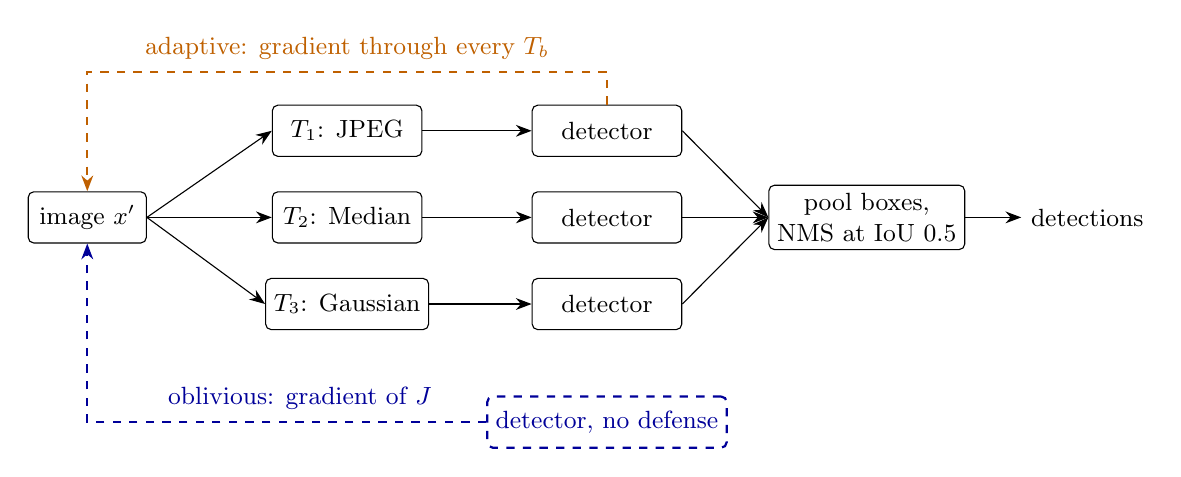
\begin{tikzpicture}[font=\small, >={Stealth[length=2mm]},
  box/.style={draw, rounded corners=2pt, minimum height=6.5mm,
              minimum width=19mm, inner sep=3pt},
  obl/.style={blue!60!black, dashed, thick},
  ada/.style={orange!75!black, dashed, thick}]
\node[box, minimum width=15mm] (x) at (0,0) {image $x'$};
\node[box] (t1) at (3.3,1.1) {$T_1$: JPEG};
\node[box] (t2) at (3.3,0) {$T_2$: Median};
\node[box] (t3) at (3.3,-1.1) {$T_3$: Gaussian};
\node[box] (f1) at (6.6,1.1) {detector};
\node[box] (f2) at (6.6,0) {detector};
\node[box] (f3) at (6.6,-1.1) {detector};
\node[box, align=center] (m) at (9.9,0) {pool boxes,\\NMS at IoU 0.5};
\node (o) at (12.7,0) {detections};
\foreach \i in {1,2,3} {
  \draw[->] (x.east) -- (t\i.west);
  \draw[->] (t\i) -- (f\i);
  \draw[->] (f\i.east) -- (m.west);
}
\draw[->] (m) -- (o);
% adaptive gradient: back through every branch
\draw[ada, ->] (f1.north) -- (6.6,1.85) -| (x.north);
\node[ada, solid, draw=none, anchor=south] at (3.3,1.88)
  {adaptive: gradient through every $T_b$};
% oblivious gradient: bare detector only
\node[box, obl] (fb) at (6.6,-2.6) {detector, no defense};
\draw[obl, ->] (fb.west) -| (x.south);
\node[obl, solid, draw=none, anchor=south] at (2.7,-2.57)
  {oblivious: gradient of $J$};
\end{tikzpicture}
\caption{The defense that is scored (solid) and the gradient each attacker
follows (dashed), for the ensemble EnsJMG on \yw{}. Every branch runs the
detector once on a transformed copy of the image, and a box survives the
merge if any branch keeps it. The oblivious attacker differentiates the bare
detector; the adaptive attacker differentiates an objective over all
branches, Eq.~\ref{eq:Jmax} or the average of the branch objectives
(Sec.~\ref{sec:adaptive-method}).}
\label{fig:pipeline}
\end{figure}

\subsection{Attacks}
\label{sec:attacks}

Each attack runs in the input space of its model and the result is saved as
an ordinary 8-bit image at the original resolution, because that is what a
deployed defense receives.

\paragraph{\fl{}.} The image is resized to $768\times768$ and normalized by
the ImageNet mean and standard deviation. The attack perturbs this tensor
$z$. The model first decodes the clean image; the resulting tokens
$y^{\mathrm s}_{1:T}$ serve as labels, and the attack maximizes their mean
cross-entropy under teacher forcing,
\begin{equation}
\mathcal{L}_{\mathrm{F}}(z') = -\frac1T\sum_{t=1}^{T}
 \log p_\theta\big(y^{\mathrm s}_t \mid y^{\mathrm s}_{<t}, z', q\big),
\end{equation}
where $q$ is the task prompt. No ground truth is involved.

\paragraph{\yw{}.} The image is letterboxed to $640\times640$ and the attack
perturbs this tensor in $[0,1]$. \yw{} has no tokens, so the objective is
different: with $s_{a,c}(z)$ the class score of anchor $a$ for class $c$
after the sigmoid and before non-maximum suppression, the attack minimizes
\begin{equation}
J(z') = \sum_{a} \max_{c}\, s_{a,c}(z'),
\label{eq:J}
\end{equation}
the total confidence of the most likely class at every anchor. It uses no
labels of any kind and no box term.

\paragraph{Three attacks.} FGSM~\cite{goodfellow2015explaining} takes one
signed gradient step of size $\epsilon$. PGD~\cite{madry2018towards} takes
10 steps of size $\epsilon/4$ from a uniform random start, projecting onto
the $\linf$ ball after each. These are the settings of every oblivious run in
Secs.~\ref{sec:damage} to~\ref{sec:rq2}; the adaptive experiment has its own
(Sec.~\ref{sec:adaptive-method}). The patch attack~\cite{brown2017adversarial}
optimizes a $35\times35$ square at the center of the attack tensor for 100
Adam steps (learning rate 0.02). Its pixels are limited only to the valid
range, not to an $\epsilon$-ball. It is a digital patch, computed per
image, with no expectation over placement or lighting and no printability
term, so we make no claim about physical attacks.

\paragraph{Budgets differ between the models.} We use $\epsilon=0.03$ in
each model's attack space. For \yw{} that is 7.65 gray levels out of 255.
For \fl{}, whose attack space is normalized, it is about 1.7 gray levels,
4.4 times less. Attack strength is therefore not comparable across the two
models, and every conclusion below is drawn within a model.

\paragraph{From attack space to image.} After the attack, the tensor is
converted to 8 bits by truncation and resized back to the original
resolution with bicubic interpolation. The $\linf$ bound holds exactly in
the attack space and only approximately in the saved image.
Sec.~\ref{sec:adaptive-method} describes a variant without the resize.

\subsection{Defenses}

Table~\ref{tab:params} lists the transforms. Parameters were fixed before
the evaluation and are the same for both models; nothing was tuned per model
or per attack.

\begin{table}[t]
\centering\small
\caption{Input transforms and parameters, identical for both models.}
\label{tab:params}
\begin{tabular}{@{}ll@{}}
\toprule
Transform & Parameters \\
\midrule
JPEG~\cite{dziugaite2016study} & quality 75 \\
Median~\cite{xu2018feature} & $3\times3$ window \\
Gaussian & $\sigma=1$ \\
Bit-depth~\cite{xu2018feature} & 4 bits per channel \\
Ordered dithering & $4\times4$ Bayer matrix, 16 levels \\
TVM~\cite{chambolle2004algorithm,guo2018countering} & weight 0.05, 200 iterations \\
Blur+TVM & Gaussian ($\sigma=1$), then TVM \\
Non-local means~\cite{buades2005non} & $h=0.8\,\hat\sigma$, $5\times5$ patches \\
SVD & per channel, top 90\% of singular values by count \\
Bilateral~\cite{tomasi1998bilateral} & $\sigma_s=1$, $\sigma_r=0.1$ \\
Anisotropic diffusion~\cite{perona1990scale} & 5 iterations, $\kappa=0.05$ \\
BM3D~\cite{dabov2007image} (OCR only) & $\sigma=0.1$ \\
Random resize-and-pad~\cite{xie2018mitigating} (OCR only) & scale in $[0.9,1]$ \\
\bottomrule
\end{tabular}
\end{table}

\paragraph{Output-level ensembles.} An ensemble of $k$ transforms runs the
model $k$ times, once per transformed image. For detection, the boxes of all
branches are pooled and greedy class-aware non-maximum suppression at IoU 0.5
keeps the highest-scoring box of each overlapping group. A box that only one
branch produces therefore survives. For OCR there are no boxes to merge; the
ensemble returns the string that at least two branches agree on, or otherwise
the branch output most similar to the others. We name ensembles by their
members: EnsJMG is JPEG, Median and Gaussian; EnsJMT replaces Gaussian by
TVM; Ens4W uses all four; EnsBTC is JPEG, Blur+TVM and Median. An ensemble
costs $k$ forward passes, and that cost is part of any fair comparison with
a single transform.

\subsection{What a reader needs to know about the measurements}
\label{sec:disclosures}

\paragraph{\fl{} detection scores are assigned by us.} The \texttt{<OD>}
output has boxes and labels but no confidences, and mAP needs a ranking. We
give each box a score between 0.6 and 0.98 that grows with its area and with
its closeness to the image center. The same rule is applied in every
condition, so differences between conditions are meaningful, but the
absolute \fl{} mAP ranks boxes by geometry and should not be compared with
\yw{}'s. To check that conclusions do not hinge on this rule we also compute
precision, recall and F1 at IoU 0.5, which use no score, and quote them where
they bear on a claim.

\paragraph{The OCR number is self-consistency.} COCO has no text
annotations. For OCR we compare the text read from an attacked or defended
image with the text the same model read from the clean image, using the
character-level matching ratio of Python's \texttt{difflib}. The clean value
is 1 by construction. A wrong reading that survives an attack scores 1, and
an image with no text scores 1 whenever the model again outputs nothing. The
number measures how stable the output is, not whether it is right.

\paragraph{Random resize-and-pad is excluded from detection.} Our
implementation shrinks the image and pastes it at an offset without mapping
the predicted boxes back, so its detection scores measured a misalignment and
not the defense. We report it for OCR only.

\paragraph{Uncertainty.} For the 1{,}000-image set we draw 1{,}000 bootstrap
resamples of images~\cite{efron1993introduction}, use the same resamples for
every condition, and report 95\% percentile intervals of paired differences
(defended minus attacked, defended-clean minus clean, ensemble minus
single transform). We also compute the bias-corrected percentile
interval~\cite{efron1993introduction}. It reaches the same verdict as the
plain interval in every cell of Tables~\ref{tab:ci-yolo}
and~\ref{tab:ci-florence}; the one comparison in the text where the two
disagree is flagged in Sec.~\ref{sec:rq2}. These intervals cover the choice
of images only. Each
oblivious condition was attacked once, so randomness in the PGD start is not
included; Sec.~\ref{sec:adaptive} uses three seeds.

\subsection{The adaptive attack}
\label{sec:adaptive-method}

The adaptive attacker targets a specific defense with branches
$T_1,\dots,T_k$ (for a single transform, $k=1$). On the forward pass each
branch computes exactly what the deployed defense computes, including its
8-bit conversion. On the backward pass we need a gradient through $T_b$:
\begin{itemize}
\item Gaussian: the true gradient (it is a convolution).
\item Median: the true gradient almost everywhere. Each output pixel passes
its gradient to the one input pixel its window selected.
\item JPEG and TVM: the identity, the standard BPDA
choice~\cite{athalye2018obfuscated}.
\item Blur+TVM: the true gradient of the Gaussian, then the identity through
TVM.
\end{itemize}
The 8-bit conversion inside each branch is passed straight through.

With several branches the usual EOT objective averages the branch losses.
That is the wrong target for a merge that keeps a box when \emph{any} branch
keeps it: pushing the average down can leave one branch confident, and that
branch's box survives. Because every branch reaches the model at the same
resolution, anchors line up across branches, and we can ask for what the
merge requires:
\begin{equation}
J_{\max}(z') = \sum_{a}\; \max_{b\le k}\; \max_{c}\; s_{a,c}\big(T_b(z')\big).
\label{eq:Jmax}
\end{equation}
At every anchor only the most confident branch contributes. This is still a
proxy, since the real merge matches boxes by overlap after thresholding and
not anchors by index. We expected it to be the stronger objective for this
merge rule; on \yw{} it was not (Sec.~\ref{sec:adaptive}). We therefore run
both Eq.~\ref{eq:Jmax} and the average over branches against every ensemble
and report, for each defense, the lower of the two defended mAPs. Neither
objective is new.

In this experiment the oblivious and the adaptive attack run side by side on
the same images. Both start from the same seeded random point for a given
image, so they differ only in the gradient they follow. Both optimize the
image at its original resolution through a differentiable copy of the
detector's own letterbox, so that each transform acts at the scale at which
it is deployed and nothing resamples the perturbation afterwards. The result
is converted to 8 bits by truncation and clipped to $\pm7$ gray levels of the
clean image, so no pixel the defense receives moves by more than $\epsilon$.
Because of this change of attack space, the oblivious numbers of
Table~\ref{tab:adaptive} are not the ones of Sec.~\ref{sec:rq2}. We run
50 steps of size $\alpha=0.002$ (about $\epsilon/15$) with one restart, on
the first 1{,}000 images. Within
a restart we keep whichever of the last iterate and the lowest-objective
iterate seen during the run has the lower objective after the 8-bit
conversion, and across restarts the restart whose result has the lowest
objective. Both attacks use this rule, each with its own objective.

\paragraph{\fl{}.} The same experiment runs on \fl{} detection with the
loss $\mathcal{L}_{\mathrm F}$ of Sec.~\ref{sec:attacks} in place of $J$:
the attacker maximizes the cross-entropy of the clean decode, through each
branch with the same backward rules. With several branches the counterpart
of Eq.~\ref{eq:Jmax} raises, at every step, the cross-entropy of the branch
that still agrees best with the clean decode,
$\min_{b\le k}\mathcal{L}_{\mathrm F}(T_b(z'))$, since a box survives the
merge as long as one branch keeps it. Unlike the \fl{} attacks of
Sec.~\ref{sec:attacks}, this one perturbs the image itself, at its original
resolution and in $[0,1]$, and reaches the model through a differentiable
copy of the processor's resize and normalization. Its budget is therefore
the same $\pm7$ gray levels as for \yw{}, about four times the budget of
the earlier \fl{} runs, and its numbers are not comparable with
Tables~\ref{tab:ci-florence} and~\ref{tab:full-florence}. Scored inference
still decodes with beam search, which the attack does not differentiate
through.

% ======================================================================
\section{Results}

\subsection{Attack damage}
\label{sec:damage}

\begin{table}[t]
\centering\small
\caption{Undefended models on COCO val2017, 5{,}000 images. Detection: mAP.
OCR: self-consistency (Sec.~\ref{sec:disclosures}). Columns are not
comparable across models (Sec.~\ref{sec:attacks}).}
\label{tab:damage}
\begin{tabular}{@{}lccc@{}}
\toprule
 & \yw{} detection & \fl{} detection & \fl{} OCR \\
\midrule
Clean & 0.452 & 0.330 & 1.000 \\
FGSM & 0.205 & 0.249 & 0.346 \\
PGD & 0.062 & 0.201 & 0.294 \\
Patch & 0.426 & 0.296 & 0.383 \\
\bottomrule
\end{tabular}
\end{table}

Table~\ref{tab:damage} shows each attack with no defense. PGD does the most
damage in every column. The patch does little to detection: 0.026 mAP on
\yw{} and 0.034 on \fl{}. That matters for everything said about the patch
below, because a defense cannot recover more than the attack removed, and
recovery expressed as a percentage of 0.026 mAP turns noise into large
numbers. We report patch results in absolute mAP.

\subsection{RQ1: what the transforms cost on clean images}
\label{sec:rq1}

\begin{table}[t]
\centering
\caption{\yw{}, first 1{,}000 images of val2017. Clean cost is mAP with the
transform on clean images minus clean mAP. Recovery is defended minus
attacked mAP. Brackets are 95\% paired bootstrap intervals; bold marks an
interval that excludes zero.}
\label{tab:ci-yolo}
\resizebox{\linewidth}{!}{%
\begin{tabular}{@{}lcccc@{}}
\toprule
 & Clean cost & FGSM recovery & PGD recovery & Patch recovery \\
\midrule
\tabinput{tab_ci_yolo}
\bottomrule
\end{tabular}}
\end{table}

\begin{table}[t]
\centering
\caption{\fl{} detection, same images and conventions as
Table~\ref{tab:ci-yolo}. Scores are the geometric pseudo-scores of
Sec.~\ref{sec:disclosures}.}
\label{tab:ci-florence}
\resizebox{\linewidth}{!}{%
\begin{tabular}{@{}lcccc@{}}
\toprule
 & Clean cost & FGSM recovery & PGD recovery & Patch recovery \\
\midrule
\tabinput{tab_ci_florence}
\bottomrule
\end{tabular}}
\end{table}

The first column of Tables~\ref{tab:ci-yolo} and~\ref{tab:ci-florence}
answers RQ1 for the five transforms and three ensembles whose per-image
outputs we kept.

On \yw{} nothing is free. Every transform lowers clean mAP by an amount whose
interval excludes zero: between 0.015 (Gaussian) and 0.029 (TVM) for single
transforms, 0.062 for Blur+TVM, and between 0.009 and 0.012 for the
ensembles. The ensembles cost least, plausibly because the merge lets the least damaged
branch speak for each object.

\fl{} splits in two. JPEG, Median and all three ensembles cost less than
0.01 mAP, with intervals that include zero. TVM, Gaussian and Blur+TVM cost
0.07 to 0.10 mAP, 19 to 26\% of the model's clean score. The
score-free metrics agree: those three lose 0.07 to 0.10 F1 on clean images.
Whatever these smoothing filters remove, \fl{} needs it and \yw{} mostly does
not.

\begin{table}[t]
\centering\small
\caption{Clean cost of every transform on all 5{,}000 images, one run, no
intervals. Detection: defended minus undefended clean mAP (\yw{} 0.452,
\fl{} 0.330). OCR: self-consistency of the defended clean output, which is
1 without a defense. Random resize-and-pad and BM3D are scored on OCR only
(Sec.~\ref{sec:disclosures}).}
\label{tab:clean5000}
\begin{tabular}{@{}lccc@{}}
\toprule
 & \yw{} & \fl{} detection & \fl{} OCR \\
\midrule
\tabinput{tab_clean_n5000}
\bottomrule
\end{tabular}
\end{table}

Table~\ref{tab:clean5000} extends this to every transform and ensemble on
all 5{,}000 images. The pattern holds. On \yw{} every single transform
except SVD, which keeps 90\% of the singular values and is close to the
identity, costs mAP: 0.002 (non-local means) to 0.057 (Blur+TVM). Every
ensemble costs less than each of its members, between 0.004 and 0.010,
except EnsJTS, which costs nothing, as does its member SVD. On \fl{} the
same smoothing filters are again the expensive ones (Gaussian 0.056, TVM
0.066, Blur+TVM 0.081, and bit-depth reduction 0.050), while every ensemble
costs at most 0.010. OCR is where nothing is cheap. On clean images the
defended reading agrees with the undefended one at between 0.51 (Blur+TVM)
and 0.95 (SVD), Median reaches 0.62, and no ensemble exceeds 0.85. Whatever
a transform recovers on the OCR track under attack, it starts from this
ceiling.

\subsection{RQ2: recovery against oblivious attacks}
\label{sec:rq2}

\paragraph{The patch supports no positive claim.} In neither model does any
transform or ensemble have a patch-recovery interval above zero
(last column of Tables~\ref{tab:ci-yolo} and~\ref{tab:ci-florence}). Several
are significantly negative, and here the clean-cost column explains what the
earlier version of this work could only guess at. In all six significantly
negative cases (JPEG, TVM and Blur+TVM on \yw{}; TVM, Gaussian and Blur+TVM
on \fl{}) the loss under the patch is no larger than the same transform's
loss on clean images (Figure~\ref{fig:cost-patch}). A patch that removes 0.023 mAP (\yw{}) or 0.034 mAP
(\fl{}) on these images leaves an image that is, for the detector, almost
clean, and a filter applied to it pays
its usual price and gets nothing back. These transforms are not being
defeated by the patch. There is too little damage for them to undo.

\begin{figure}[t]
\centering
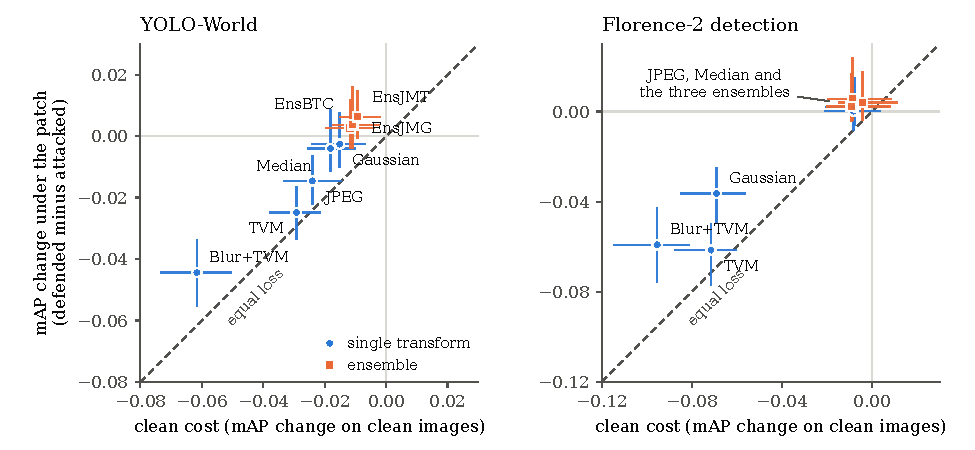
\includegraphics[width=\linewidth]{fig_cost_vs_patch.pdf}
\caption{Clean cost against the mAP change under the patch, first 1{,}000
images, for the eight defenses of Tables~\ref{tab:ci-yolo}
and~\ref{tab:ci-florence}. Bars are 95\% paired bootstrap intervals. On the
dashed line a transform loses as much on patched images as on clean ones.
Every defense lies on or above it: none loses more under the patch than it
already loses without an attack.}
\label{fig:cost-patch}
\end{figure}

\paragraph{Ensembles beat Median on \yw{} only.}
Median is the one single transform that is never significantly harmful
under any of the six attacked settings, so it is the natural baseline for
the ensembles. On \yw{} the best
ensemble exceeds Median by 0.044 mAP under FGSM, 0.049 under PGD (interval
0.039 to 0.059) and 0.010 under the patch (0.002 to 0.016). On \fl{} the
corresponding gaps are 0.009, 0.005 and 0.004. Only the FGSM gap has a
percentile interval that excludes zero (0.0003 to 0.018), and it does not
once the bootstrap's small-sample bias is corrected. The claim that merging
at the output level beats a single filter is therefore a statement about
\yw{}. On \fl{}, two extra forward passes buy no mAP we can measure over a
median filter. At the looser AP50 the same three gaps are 0.017 to 0.022 and
all three intervals exclude zero, so this negative result holds for mAP only.

Median is not the strongest single transform in every column, and against
the strongest one the ensembles' lead on \yw{} is smaller or absent. Under
FGSM, Blur+TVM (0.345) is ahead of every ensemble (best 0.336), at a clean
cost of 0.062; under PGD the best ensemble (0.413) leads Gaussian (0.405) by
0.008. We did not compute intervals for these two comparisons.

\paragraph{The same transform can help one model and hurt the other.}
TVM is among the best single transforms on \yw{} under PGD ($+0.331$) and is
indistinguishable from useless on \fl{} under FGSM ($-0.010$, interval
includes zero). The clean-cost column again accounts for most of it: TVM
costs \fl{} 0.071 mAP before any attack, and a transform that starts 0.07
behind has to remove a great deal of damage to end up ahead.

\paragraph{How fragile is the oblivious perturbation?} Under PGD, \yw{}
falls from 0.476 to 0.074 mAP on the 1{,}000-image set. A $3\times3$ median
filter, the mildest transform we tested, brings it back to 0.364, which is
72\% of the loss. Gaussian blur reaches 0.405 against 0.461 for the same
blur on clean images, leaving 0.056 mAP of damage. We do not read this as
evidence that a median filter is a strong defense. It shows that ten steps
of PGD against the bare model produce a perturbation that barely survives
any change to the image, and that is exactly the situation in which
oblivious numbers are least informative. It is the reason for RQ3.

\paragraph{The full table.} Appendix~\ref{app:full} gives all transforms on
5{,}000 images, without intervals. The two image sets differ in detail, as the intervals lead one to
expect: Median's small patch recovery on \yw{}, for example, is positive on
5{,}000 images and slightly negative on the first 1{,}000.

\subsection{RQ3: an attacker who knows the defense}
\label{sec:adaptive}

\begin{table}[t]
\centering\small
\caption{\yw{} under oblivious and adaptive PGD, first 1{,}000 images,
$\epsilon=7/255$, 50 steps; clean mAP 0.476. Each row is one target defense;
the adaptive attack is computed against that defense. The first five columns
use the objective of Eq.~\ref{eq:Jmax}; Median and EnsJMG are the mean over
three seeds (standard deviation), Ens4W is one seed. The last column is the
adaptive attack with the average objective (seed 1); for a single transform
the two objectives coincide. Both attacks optimize at the original
resolution (Sec.~\ref{sec:adaptive-method}), so the oblivious columns are not
those of Table~\ref{tab:ci-yolo}.}
\label{tab:adaptive}
\resizebox{\linewidth}{!}{%
\begin{tabular}{@{}lcccccc@{}}
\toprule
 & & \multicolumn{2}{c}{Oblivious PGD} & \multicolumn{3}{c}{Adaptive PGD} \\
\cmidrule(lr){3-4}\cmidrule(lr){5-7}
 & Clean, & & & & defended & defended \\
Target & defended & undefended & defended & undefended & (Eq.~\ref{eq:Jmax}) & (average) \\
\midrule
\tabinput{tab_adaptive_yolo}
\bottomrule
\end{tabular}}
\end{table}

Table~\ref{tab:adaptive} is read row by row. The honest comparison is between
worst cases: the defended model under whichever attack hurts it most, against
the undefended model under whichever attack hurts it most. An adaptive
perturbation is tuned to the defense and may be a weaker attack on the bare
model, so comparing the two ``adaptive'' columns alone would flatter the
defense.

The adaptive attack takes back almost everything the defenses gave. Under
oblivious PGD the three defenses hold 0.366, 0.407 and 0.431 mAP. Against an
attacker who targets them, the worst case over the two objectives (seed 1)
is 0.016 for Median, 0.048 for EnsJMG and 0.069 for Ens4W, while the
undefended model under the same attack has 0.018. Median ends where no
defense would. The ensembles keep 0.030 and 0.050 mAP more than that, which
is an advantage over Median, but a small one next to a clean mAP of 0.476.
The column ``adaptive, undefended'' shows why the comparison has to be
between worst cases: the perturbation tuned against Median barely hurts the
bare model (0.452), so a reader who compared the two adaptive columns would
credit Median with almost nothing to defend against. The three seeds agree
closely: with Eq.~\ref{eq:Jmax}, Median's defended mAP lies between 0.016
and 0.019 and EnsJMG's between 0.071 and 0.075.

Against its own members the ensemble's lead is small. Table~\ref{tab:budget}
repeats the attack on the first 300 images for JPEG and Gaussian alone. At
$7/255$ EnsJMG keeps 0.066 under the adaptive attack, against 0.062 for JPEG,
0.035 for Gaussian and 0.022 for Median. It ends level with its strongest
member, and that member is the one whose gradient we approximate by the
identity, the part of our attack most likely to be too weak
(Sec.~\ref{sec:adaptive-method}).

\begin{table}[t]
\centering\small
\caption{Defended mAP against the attack budget, first 300 images, 50 steps,
seed 1. For each budget: oblivious PGD, then the adaptive attack against that
defense (for EnsJMG, the worse of the two objectives). The ``no defense'' row
is oblivious PGD on the bare model in both columns. The $7/255$ entries of
Median and EnsJMG are the first 300 images of the runs of
Tables~\ref{tab:adaptive} and~\ref{tab:adaptive-florence}. \fl{}'s undefended
cells are the mean of two runs that differ by 0.004 ($7/255$) and 0.001
($4/255$) (Sec.~\ref{sec:adaptive}).}
\label{tab:budget}
\begin{tabular}{@{}llcccc@{}}
\toprule
 & & \multicolumn{2}{c}{$\epsilon=4/255$} & \multicolumn{2}{c}{$\epsilon=7/255$} \\
\cmidrule(lr){3-4}\cmidrule(lr){5-6}
Model & Defense & oblivious & adaptive & oblivious & adaptive \\
\midrule
\tabinput{tab_budget}
\bottomrule
\end{tabular}
\end{table}

\paragraph{Checks.} Following~\cite{carlini2019evaluating}, we verify that
the attack is doing what it should.
(i) Measured through the target defense, the adaptive attack reaches a lower
value of its objective than the oblivious attack on 999 or 1{,}000 of the
1{,}000 images in every run.
(ii) The attack has not converged at 50 steps. On the first 300 images,
EnsJMG falls from 0.086 after 50 steps to 0.054 after 100. Every adaptive
number in this section is therefore an upper bound on what the defense
keeps.
(iii) A larger budget drives the defended mAP toward zero: at
$\epsilon=25/255$ ($\epsilon=0.1$, $\alpha=0.0067$) EnsJMG keeps 0.023 under
the adaptive attack, against 0.340 under the oblivious one, on the same 300
images. At a smaller budget the defenses keep more, and the ensemble keeps
most (Table~\ref{tab:budget}). At $4/255$, where oblivious PGD leaves the
undefended \yw{} at 0.062, the adaptive attack leaves Median at 0.054,
Gaussian at 0.082, JPEG at 0.126 and EnsJMG at 0.137 (0.174 with
Eq.~\ref{eq:Jmax}, 0.137 with the average). Median is again at the
undefended level; EnsJMG keeps 0.075 mAP above it, 0.011 more than JPEG
alone. On \fl{} at $4/255$, where the undefended model keeps 0.195, Median
keeps 0.214 and EnsJMG 0.256 under the adaptive attack (EnsJMG with the
merge-specific objective only, which matched the average at $7/255$), that
is 0.019 and 0.061 above no defense, against $-0.004$ and 0.030 on the same
images at $7/255$. On both models the defenses keep more as the budget
shrinks, and the ensemble's margin grows with it; none of them comes close
to its oblivious number at either budget.
(iv) Eq.~\ref{eq:Jmax} is the weaker objective on \yw{}. With the average
over branches, EnsJMG falls to 0.048 instead of 0.071 and Ens4W to 0.069
instead of 0.108 (seed 1). On \fl{} the two give the same result for EnsJMG
on its first 300 images (0.199 with the merge-specific objective, 0.201 with
the average). A plausible reason is that the anchor-wise maximum passes the
gradient of only one branch at each anchor, while the average moves every
branch at every step; within 50 steps that matters more than aiming at the
branch the merge will keep. This is why every worst case above takes the
minimum over both.
(v) The true median gradient is the stronger choice: with it Median falls to
0.016, with the straight-through identity to 0.042 (seed 1).

\begin{table}[t]
\centering\small
\caption{\fl{} detection under oblivious and adaptive PGD, first 1{,}000
images, $\epsilon=7/255$ in pixel space, 50 steps, one seed; clean mAP 0.360.
Columns as in Table~\ref{tab:adaptive}. The average objective was run for
EnsJMG on the first 300 images only (check iv). Geometric pseudo-scores
(Sec.~\ref{sec:disclosures}).}
\label{tab:adaptive-florence}
\resizebox{\linewidth}{!}{%
\begin{tabular}{@{}lcccccc@{}}
\toprule
 & & \multicolumn{2}{c}{Oblivious PGD} & \multicolumn{3}{c}{Adaptive PGD} \\
\cmidrule(lr){3-4}\cmidrule(lr){5-7}
 & Clean, & & & & defended & defended \\
Target & defended & undefended & defended & undefended & (merge obj.) & (average) \\
\midrule
\tabinput{tab_adaptive_florence}
\bottomrule
\end{tabular}}
\end{table}

\paragraph{\fl{}.} Table~\ref{tab:adaptive-florence} repeats the experiment
on \fl{} detection. The pattern is the same and the numbers are less
extreme, because the attack itself does less damage to this model: oblivious
PGD at the same budget leaves the undefended model at 0.134 to 0.138. Under
that attack Median and EnsJMG add 0.12 and 0.13 mAP (0.256 and 0.264). Under
the adaptive attack they hold 0.148 and 0.166, so they keep 0.010 and 0.032
mAP above the undefended model. The adaptive objective was lower than the
oblivious one, measured through the target, on every image. \fl{} runs are
not repeatable bit for bit on our GPU: the undefended oblivious cell, which
the two rows compute from the same seed and images, differs by 0.005 between
them, and differences of that size in this table are noise.

\subsection{A third model}
\label{sec:third}

Whether a transform chosen on two detectors carries over to a model of a
different kind is a fair question for a defense that is meant to be attached
to any model. We therefore fixed one more model before running anything on
it: SmolVLM-256M-Instruct~\cite{marafioti2025smolvlm}, a chat-style vision-language model with 0.26
billion parameters. It returns text, not boxes, so the task changes. For
each image we ask yes/no questions of the form ``Is there a \emph{class} in
this image?'', half about a COCO class annotated in the image and half about
one that is not, and score accuracy against the annotations; the answer is
read from the next-token probabilities of ``yes'' and ``no''. The attack is
oblivious PGD ($\epsilon=0.03$ on the image, 10 steps) that maximizes the
cross-entropy of the correct answers. An ensemble answers with the mean of
its branches' yes-probabilities. Every image is resized to the model's
$512\times512$ input in every condition, so the transforms act at that
size. No adaptive attack was run on this model.

\begin{table}[t]
\centering\small
\caption{SmolVLM-256M, yes/no presence questions on the first 1{,}000
images (2{,}000 questions, 49.6\% with answer yes). Accuracy without a
defense: 0.856 clean, 0.439 under oblivious PGD. Clean cost is defended
minus undefended clean accuracy; recovery is defended minus undefended
attacked accuracy. Brackets are 95\% paired bootstrap intervals over images;
bold marks an interval that excludes zero. Sorted by attacked accuracy.}
\label{tab:smolvlm}
\resizebox{\linewidth}{!}{%
\begin{tabular}{@{}lcccc@{}}
\toprule
 & Clean acc. & Clean cost & Attacked acc. & Recovery \\
\midrule
\tabinput{tab_smolvlm}
\bottomrule
\end{tabular}}
\end{table}

Table~\ref{tab:smolvlm} gives the result. The attack lowers accuracy from
0.856 to 0.439. The ranking is not the one the detectors gave. The strongest
smoothing filters recover most of the loss: Blur+TVM reaches 0.754,
random resize-and-pad 0.748 and BM3D 0.728, between 69 and 75\% of the
damage, at clean costs of 0.03 to 0.07. Median recovers 0.093 (22\%), and the
seven ensembles between 0.032 and 0.100 (8 to 24\%). Every ensemble here is
below its own best member under attack; averaging the yes-probabilities
lets the weak branches dilute the strong one, where the detection merge lets
the strong branch's boxes through. Four transforms (non-local means,
dithering, SVD, bit-depth reduction) neither cost nor recover anything we
can measure. Since no adaptive attack was run here, these recoveries are
upper bounds in the sense of Sec.~\ref{sec:adaptive}.

\subsection{A fourth model}
\label{sec:fourth}

The third model changes the task as well as the architecture, so it cannot
say whether the ensembles' behavior on the two detectors is a property of
detection or of those two models. We therefore added a second
open-vocabulary detector with a different design, chosen before any of its
results were seen: OWL-ViT~\cite{minderer2022simple}
(\texttt{google/owlvit-base-patch32}, about 150 million parameters), which
puts a box and a score for every text query on each of the 576 patches of a
CLIP vision transformer. It has real confidences, so its mAP is ranked by
score as \yw{}'s is. We prompt it with ``a photo of a \emph{class}'' for the
80 COCO classes, keep boxes scoring at least 0.001 after class-aware
non-maximum suppression at IoU 0.5 and at most 300 per image, the settings
we use for \yw{}. Both attacks minimize the objective of Eq.~\ref{eq:J} with
$s_{a,c}$ the sigmoid score of patch $a$ for query $c$, in pixel space at
the original resolution with the budget, steps and objectives of
Sec.~\ref{sec:adaptive-method}; patches line up across branches because
every branch is resized to the same $768\times768$ input.

\begin{table}[t]
\centering\small
\caption{OWL-ViT under oblivious PGD ($\epsilon=7/255$, 50 steps), first
1{,}000 images; clean mAP 0.310, attacked 0.012. Clean cost is defended minus
undefended clean mAP; recovery is the share of the attack's damage that the
defense restores. Last column: an ensemble's attacked mAP minus that of its
best member, with a 95\% paired bootstrap interval over images (1{,}000
resamples); bold marks an interval that excludes zero. Sorted by attacked
mAP.}
\label{tab:owl}
\resizebox{\linewidth}{!}{%
\begin{tabular}{@{}lcccl@{}}
\toprule
 & Clean cost & Attacked mAP & Recovery & Ensemble minus best member \\
\midrule
\tabinput{tab_owl_survey}
\bottomrule
\end{tabular}}
\end{table}

Table~\ref{tab:owl} is the one setting in this paper where the ensembles do
what they were built to do. PGD lowers OWL-ViT from 0.310 to 0.012 mAP.
Every ensemble ends above each of its own members, and for six of the seven
the interval of that difference excludes zero; the margins are small, 0.003
to 0.009 mAP. Every ensemble also leads Median, by 0.032 to 0.075 mAP, with
intervals that exclude zero. On clean images no ensemble costs anything we
can measure (point estimates $+0.002$ to $+0.006$, every interval includes
zero), while every single transform except SVD costs mAP, from less than
0.001 (non-local means) to 0.042 (Blur+TVM). The best single transform overall, Blur+TVM (0.236), is still
ahead of five of the seven ensembles, at that clean cost of 0.042.

The adaptive attack removes this advantage as it did on the other two
detectors. Median falls from 0.169 under oblivious PGD to 0.021, against
0.011 for the undefended model under the same attack. EnsJMG falls from
0.201 to 0.061 with the objective of Eq.~\ref{eq:Jmax}. On the first 300
images the average objective is again the stronger one: it leaves EnsJMG at
0.073, against 0.083 for Eq.~\ref{eq:Jmax} on the same images, 0.223 under the
oblivious attack and 0.012 with no defense. EnsJMG thus keeps about 0.05 mAP
more than the undefended model and 0.04 more than Median, a small margin as
on \yw{}, and its lead against oblivious attacks does not protect it here. In every run the adaptive attack reached a lower
value of its objective than the oblivious one on every image. Like \fl{},
OWL-ViT does not repeat bit for bit on our GPU: the undefended oblivious
cell, computed from the same seed and images, is between 0.0108 and 0.0117
in the three runs that contain it.

% ======================================================================
\section{Discussion}

\paragraph{FGSM and PGD.} Against oblivious attacks, transforms recover more
of the PGD damage than of the FGSM damage. Part of that is arithmetic: PGD
removes more, so there is more to give back. On \fl{} it is all arithmetic,
since the best defended mAP is almost the same under both attacks (0.328 and
0.324).
On \yw{} it is not. The best defended mAP under FGSM is 0.345, against 0.413
under PGD, so the single-step perturbation really is harder to filter out.
We can think of two explanations and have tested neither. A single large
step may put more of its energy into low spatial frequencies, which
smoothing leaves alone. Or the ten-step perturbation may simply be fitted
more closely to the bare model, and so transfer worse to the model behind a
filter, as multi-step attacks are known to transfer worse between
models~\cite{kurakin2017adversarial}. Measuring the spectra of the two
perturbations would separate them.

\paragraph{What we would recommend.} Less than the earlier version did,
and nothing against an attacker who knows the defense. On \yw{}, an
ensemble such as EnsJMG costs about 0.005 to 0.01 mAP on clean images and
three forward passes, and against attacks crafted on the bare model it is
better than a median filter, the one single filter that never did
significant harm. Table~\ref{tab:adaptive} limits what that is worth: once
the attacker accounts for it, the ensemble keeps 0.05 to 0.07 of a clean
0.48 mAP. It still keeps more than Median, so among these transforms it
remains the one to choose, but as protection against unaware attackers
only. OWL-ViT is the strongest case for an ensemble: there every ensemble
beats each of its members against oblivious attacks at no measurable clean
cost (Table~\ref{tab:owl}), so an ensemble is the right choice among input
transforms for that model, with the same caveat. On \fl{}, a median filter does as well in mAP as any ensemble we tried
at a third of the compute, and TVM and Gaussian blur should be avoided
because of what they cost on clean images. Against the patch as we
implemented it, we cannot recommend anything. A deployer who needs
robustness to an informed attacker needs something other than input
filtering; the classifier literature points to adversarial training or
heavier purification~\cite{nie2022diffusion,raber2025keep}, neither of which
we evaluated.

% ======================================================================
\section{Limitations}

The \fl{} mAP depends on scores we assign. The score-free F1 agrees with it on
the clean costs of Sec.~\ref{sec:rq1}, but a ranking by model confidence, for
instance from the token probabilities of the generated box, would be better
and is possible.

The OCR track measures stability on images that mostly contain little text.
COCO-Text~\cite{veit2016cocotext} annotates text in COCO images and would
allow accuracy to be measured on images that contain some; we have not done
this.

The patch is small, digital and weak. Our patch results say that these
filters do not help against an attack that does little damage. They say
nothing about large or physical patches, or about the dedicated patch
defenses we did not run.

The two models are attacked with budgets that differ by a factor of 4.4, so
we compare transforms within a model and never models with each other. The
adaptive evaluation covers detection on \yw{}, \fl{} and OWL-ViT; the OCR
track and SmolVLM are evaluated against oblivious attacks only. It uses the
first 1{,}000 images, 50 steps and one restart; check (ii) shows that more
steps lower the defended numbers further, so they are upper bounds, and
Ens4W and the \fl{} runs have one seed each. The identity gradient we use
for JPEG and TVM is the part of the attack most likely to be too weak
(Sec.~\ref{sec:adaptive-method}), which again makes our adaptive numbers
favorable to the defenses. We did not include a control in which
the ensemble's extra forward passes are spent on views that do not denoise
(for example a flipped or rescaled image), so we cannot say how much of the
ensemble's advantage on \yw{} comes from denoising and how much from merging
several views. And COCO is not a driving dataset; nothing here should be read
as a statement about a specific application.

% ======================================================================
\section{Conclusion}

Input transforms are the defense available to someone who deploys a frozen
open-vocabulary detector, and it is worth knowing what they are good for.
Measured against attackers who ignore them, they recover a large share of
PGD damage, at a clean cost that is small for \yw{} and, for three of the
smoothing filters, large for \fl{}. Merging the outputs of several transforms
beats a median filter on \yw{} and makes no measurable difference to \fl{}'s
mAP. No transform helps
against our patch. An attacker who knows the defense leaves little of the
rest: on \yw{} the best defense we tested keeps 0.069 of 0.476 mAP, against
0.018 with no defense; on \fl{} a defense keeps at most 0.03 mAP above
none; and on OWL-ViT, the one model on which every ensemble beats its own
members against oblivious attacks, EnsJMG keeps 0.061 of 0.310 mAP against
0.011. Input transforms, alone or merged, protect these models from attackers
who do not know they are there, and from no one else. We release the code,
the per-image outputs and the scripts that produce every table.

\bibliographystyle{plainnat}
\bibliography{refs}

% ======================================================================
\appendix
\section{All transforms on 5{,}000 images}
\label{app:full}

Tables~\ref{tab:full-yolo} to~\ref{tab:full-ocr} give every transform on the
full val2017 set under oblivious attacks, one run per condition, without
intervals. Recovery is $(\text{defended}-\text{attacked})/(\text{clean}-
\text{attacked})$ in percent. In the patch columns the denominator is 0.026
mAP (\yw{}) or 0.034 mAP (\fl{}), so percentages there magnify small
absolute changes; read the mAP column. EnsBMT is Bilateral, Median, TVM;
EnsJBT is JPEG, Bilateral, TVM; EnsJTS is JPEG, TVM, SVD.

\begin{table}[ht]
\centering\small
\caption{\yw{}, 5{,}000 images, oblivious attacks.}
\label{tab:full-yolo}
\begin{tabular}{@{}lcccccc@{}}
\toprule
 & \multicolumn{2}{c}{FGSM} & \multicolumn{2}{c}{PGD} & \multicolumn{2}{c}{Patch} \\
\cmidrule(lr){2-3}\cmidrule(lr){4-5}\cmidrule(lr){6-7}
 & mAP & Rec.\,\% & mAP & Rec.\,\% & mAP & Rec.\,\% \\
\midrule
\tabinput{tab_yolo_n5000}
\bottomrule
\end{tabular}
\end{table}

\begin{table}[ht]
\centering\small
\caption{\fl{} detection, 5{,}000 images, oblivious attacks, geometric
pseudo-scores.}
\label{tab:full-florence}
\begin{tabular}{@{}lcccccc@{}}
\toprule
 & \multicolumn{2}{c}{FGSM} & \multicolumn{2}{c}{PGD} & \multicolumn{2}{c}{Patch} \\
\cmidrule(lr){2-3}\cmidrule(lr){4-5}\cmidrule(lr){6-7}
 & mAP & Rec.\,\% & mAP & Rec.\,\% & mAP & Rec.\,\% \\
\midrule
\tabinput{tab_florence_n5000}
\bottomrule
\end{tabular}
\end{table}

\begin{table}[ht]
\centering\small
\caption{\fl{} OCR self-consistency, 5{,}000 images, oblivious attacks.}
\label{tab:full-ocr}
\begin{tabular}{@{}lccc@{}}
\toprule
 & FGSM & PGD & Patch \\
\midrule
\tabinput{tab_ocr_n5000}
\bottomrule
\end{tabular}
\end{table}

\section{Reproducibility}

All detection numbers come from \texttt{pycocotools}. The intervals in
Tables~\ref{tab:ci-yolo} and~\ref{tab:ci-florence} are computed on a CPU from
the saved detections, with no model or image loaded; the script reproduces
all 168 mAP values of the original runs exactly before resampling. PGD
starting points in the adaptive experiment are derived from a hash of the
run seed, the image id and the restart index, so the oblivious and adaptive
attacks on an image start from the same point. All Phase-4 runs use
deterministic GPU kernels where they exist. With them, repeating a \yw{}
command reproduces its saved detections bit for bit (checked on two
identical 10-image runs); \fl{} does not repeat exactly on our GPU, and two
runs from the same seed and images differ by about 0.005 mAP.
When GPU memory allows, the adaptive runs pass the $k$ defended copies of the
image through the detector as one batch, with one backward pass, per PGD
step; this is an execution option (\texttt{-{}-eot-batch}) that leaves the
objective and its gradient unchanged up to floating-point rounding. Every
run is one command of \texttt{phase4/p4\_yolo.py},
\texttt{p4\_florence.py}, \texttt{p4\_smolvlm.py} or \texttt{p4\_owl.py};
the release lists them, and \texttt{make\_phase4\_tables.py} rebuilds every
Phase-4 table from the saved summaries.

\end{document}
